\documentclass[10pt,twocolumn,letterpaper]{article}

\usepackage{dependable_dnn}
\usepackage{times}
\usepackage{epsfig}
\usepackage{graphicx}
\usepackage{amsmath}
\usepackage{amssymb}
\usepackage{bbm}
\usepackage{subfigure}
\usepackage[table, dvipsnames]{xcolor}

% Include other packages here, before hyperref.

% If you comment hyperref and then uncomment it, you should delete
% egpaper.aux before re-running latex.  (Or just hit 'q' on the first latex
% run, let it finish, and you should be clear).
\usepackage[pagebackref=true,breaklinks=true,letterpaper=true,colorlinks,bookmarks=false]{hyperref}

\DeclareMathOperator*{\argmin}{arg\,min}
\newcommand{\Rho}{\mathrm{P}}
\newcommand{\indic}[1]{\mathbbm{1}_{\{#1\}}}
\newcommand{\closs}[1]{{\cal L}_{\rm class}(#1)}
\newcommand{\bloss}[1]{{\cal L}_{\rm box}(#1)}

\iccvfinalcopy % *** Uncomment this line for the final submission

\def\iccvPaperID{} % *** Enter the Paper ID here
\def\httilde{\mbox{\tt\raisebox{-.5ex}{\symbol{126}}}}

% Pages are numbered in submission mode, and unnumbered in camera-ready
\ificcvfinal\pagestyle{empty}\fi

\begin{document}

%%%%%%%%% TITLE - PLEASE UPDATE
\title{End-to-End Object Detection with Transformers\\ {\rm {\normalsize Seungmin Lee (profile2697@gmail.com; 2020-20866), \\Dept. of Electrical and Computer Engineering, Seoul National University}}}   % **** Enter the paper title and student information here

\maketitle
\thispagestyle{empty}

\section{Introduction and Motivation}
Current object detection methods address object detection as a sequential task that predicts object classes after proposing the candidate bounding boxes (bbox). Unfortunately, this kind of approach makes the object detection pipeline complex, requiring a lot of heuristics such as Non-Maximal Suppression or a complicated training scheme~\cite{Faster}.

To address this problem, this paper treats object detection as a direct set prediction where the set is a collection of the (class, bbox) pairs. This view simplifies the object detection process by removing the task-specific heuristics. The authors implement it using a transformer that predicts (class, bbox) pairs and bipartite matching loss. 

\begin{figure}[b]
	\centering
	\subfigure[The transformer architecture]{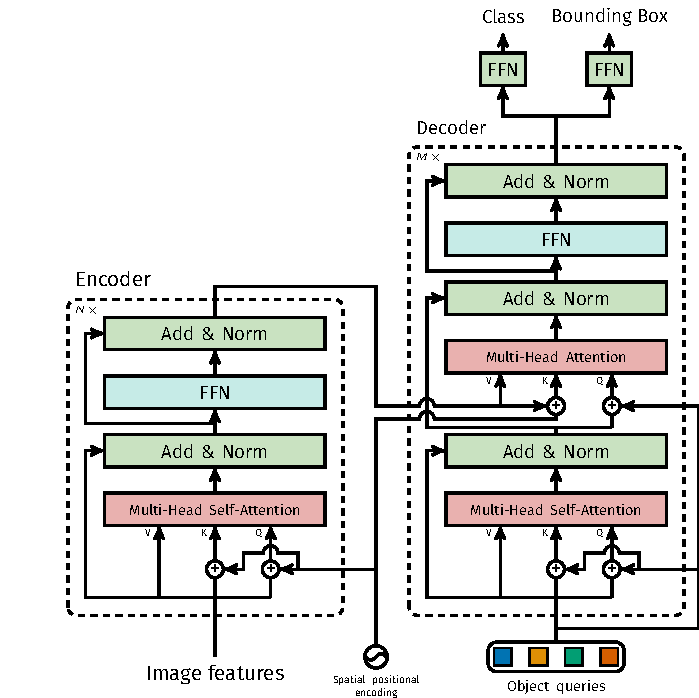
\includegraphics[width=4cm, height=2.5cm]{assets/transformer.pdf}}
	\subfigure[The encoder resolves instance occlusions]{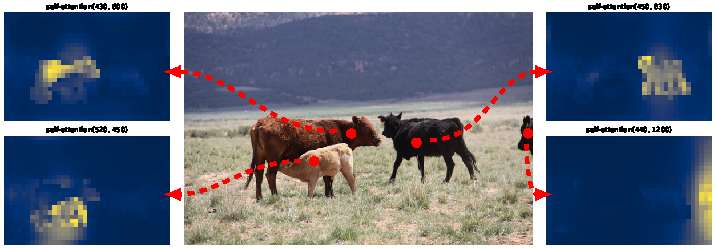
\includegraphics[width=4cm, height=2.5cm]{assets/cows_attn.pdf}}
	\caption{(a) The proposed encoder-decoder transformer architecture, (b) The encoder's attention maps: the encoder separate each instance even though those are occluded.}
	\label{fig:imgs}
\end{figure}
\vspace{-0.2cm}
\section{Method}
\subsection{Architecture: DEtection TRansformer (DETR)}
The proposed architecture named DETR consists of a CNN backbone, an encoder-decoder transformer that takes the CNN features and transforms them, and feed-forward networks that predict classes and bounding box coordinates for each token. 

When we set $N$ as a fixed prediction size, the output will be  $\hat{y} = \{\hat{y}_i\}_{i=1}^{N}$ where $\hat{y}_i = \{\hat{p}_i, \hat{b}_i\}$ is a pair of the predicted class probability ($\hat{p}_i$) and box coordinates ($\hat{b}_i$). 

The transformer has the typical form as proposed in ~\cite{SA} except they use additional positional encodings called \textit{object queries} on the decoder. The detailed architecture is shown in Figure~\ref{fig:imgs} (a). 

\subsection{Set Prediction Loss}
The proposed method calculates the loss through two steps: finding the optimal one-to-one matching between the ground truth and the set prediction, calculating loss using the found matching.

\subsubsection{Step 1: Finding the Optimal Matching}
Suppose that $y = \{c_i, b_i\}$ is the ground truth of a given image. Note that we extend $y$ to has the size $N$ by appending $\emptyset$. Thus, we can match each element of $y$ and $\hat{y}$ one-to-one. Among the possible permutation of $N$ elements ($\Rho_N$), we select the optimal permutation ($\rho^{\star}$) using the following equation:
\begin{align*}
	\rho^{\star} = \argmin_{\rho\in\Rho_N} \sum_{i=1}^{N} -\indic{c_i\neq\emptyset}\hat{p}_{\rho(i)}(c_i) + \indic{c_i\neq\emptyset} \bloss{b_{i}, \hat{b}_{\rho(i)}},
\end{align*}
where $\indic{\cdot}$ is the indicator function, and $\hat{p}_{\rho(i)}(c_i)$ is the predicted confidence of the ground truth class $c_i$. The authors utilize the Hungarian algorithm~\cite{Hung} to solve the equation effectively.

\subsubsection{Step 2: Calculating the Loss}
The proposed method uses the following loss:
\begin{align*}
	\mathcal{L}(y, \hat{y}) = \sum_{i=1}^{N} -\log\hat{p}_{\rho^{\star}(i)}(c_i) + \indic{c_i\neq\emptyset} \bloss{b_{i}, \hat{b}_{\rho(i)}}.
\end{align*}

\section{Results}
The method shows comparable or higher performance on many metrics except on the small objects. However, considering the simplicity, the performance drop seems tolerable. As we can see in Figure~\ref{fig:imgs}, the encoder attention successfully separates occluded instances. Based on the result, this paper extends their method to instance segmentation.

\section{Personal Note}
The main contributions of this paper are two-fold: object detection as a direct set prediction, integrating transformer. The first contribution seems critical because it made the object detection pipeline simple.
However, it is unclear which part of the contributions is more crucial to the performance. Therefore, it would be better to compare the proposed method with a CNN model that predicts a class-box set. 

{\small
\bibliographystyle{ieee}
\bibliography{egbib}
}


\end{document}
